\documentclass[tikz,border=6pt]{standalone}
% shared TikZ style for the diagrams (colours match the plots)
\usepackage[T1]{fontenc}
\usepackage{lmodern}
\usepackage{amsmath,amssymb}
\usepackage{tikz}
\usetikzlibrary{arrows.meta,positioning,fit,backgrounds,calc,shapes.misc,decorations.pathreplacing}
\definecolor{cBlue}{HTML}{2A78D6}
\definecolor{cOrange}{HTML}{EB6834}
\definecolor{cAqua}{HTML}{1BAF7A}
\definecolor{cViolet}{HTML}{6250D6}
\definecolor{cGreen}{HTML}{008300}
\definecolor{cGray}{HTML}{8F8D86}
\definecolor{cInk}{HTML}{0B0B0B}
\definecolor{cInk2}{HTML}{52514E}
\tikzset{
  box/.style={draw=#1!70!black, fill=#1!10, rounded corners=3pt, align=center, inner sep=4pt, font=\small, line width=0.6pt},
  box/.default=cGray,
  arr/.style={-{Stealth[length=2.4mm]}, line width=0.8pt, cInk2},
  lbl/.style={font=\scriptsize, text=cInk2, align=center},
}

\begin{document}
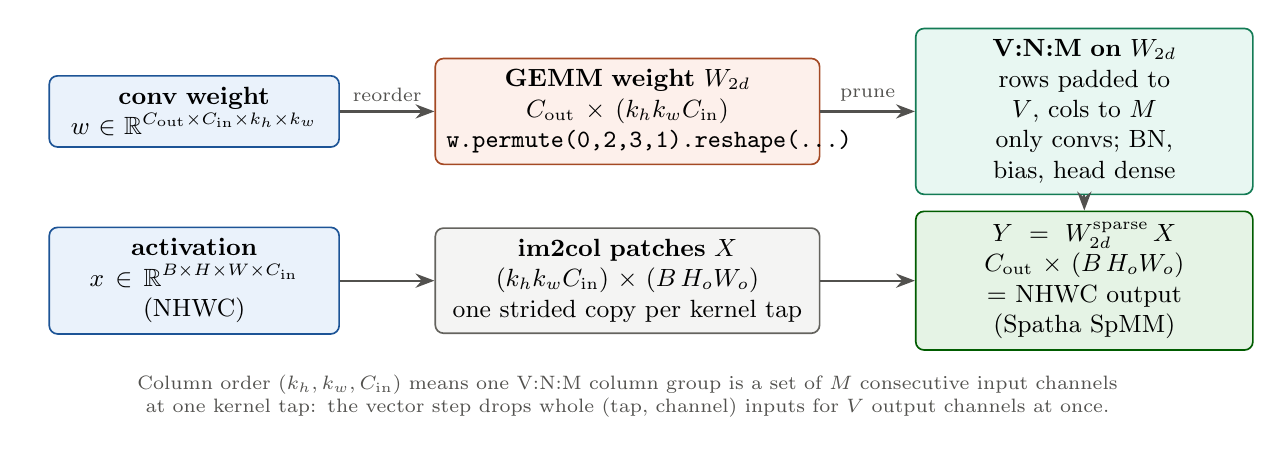
\begin{tikzpicture}[node distance=6mm and 8mm]
\node[box=cBlue, text width=34mm] (w) {\textbf{conv weight}\\$w\in\mathbb{R}^{C_\text{out}\times C_\text{in}\times k_h\times k_w}$};
\node[box=cOrange, text width=46mm, right=12mm of w] (w2) {\textbf{GEMM weight} $W_{2d}$\\$C_\text{out}\times(k_h k_w C_\text{in})$\\\texttt{w.permute(0,2,3,1).reshape(...)}};
\node[box=cAqua, text width=40mm, right=12mm of w2] (vnm) {\textbf{V:N:M on $W_{2d}$}\\rows padded to $V$, cols to $M$\\only convs; BN, bias, head dense};
\draw[arr] (w)--node[lbl,above]{reorder}(w2); \draw[arr] (w2)--node[lbl,above]{prune}(vnm);
\node[box=cBlue, text width=34mm, below=10mm of w] (x) {\textbf{activation}\\$x\in\mathbb{R}^{B\times H\times W\times C_\text{in}}$ (NHWC)};
\node[box=cGray, text width=46mm, right=12mm of x] (col) {\textbf{im2col patches} $X$\\$(k_h k_w C_\text{in})\times(B\,H_o W_o)$\\one strided copy per kernel tap};
\node[box=cGreen, text width=40mm, right=12mm of col] (y) {$Y=W_{2d}^{\text{sparse}}\,X$\\$C_\text{out}\times(B\,H_oW_o)$ = NHWC output\\(Spatha SpMM)};
\draw[arr] (x)--(col); \draw[arr] (col)--(y); \draw[arr] (vnm)--(y);
\node[lbl, text width=150mm, below=4mm of col] {Column order $(k_h,k_w,C_\text{in})$ means one V:N:M column group is a set of $M$ consecutive input channels at one kernel tap: the vector step drops whole (tap, channel) inputs for $V$ output channels at once.};
\end{tikzpicture}
\end{document}
